% Research paper, IEEE conference format (IEEEtran).
% Build:  cd reports/research_paper && latexmk -pdf paper.tex     (or: pdflatex paper.tex, twice)
% Figures are produced by ../make_figures.py from the logged runs in docs/data/.
\documentclass[conference]{IEEEtran}
\IEEEoverridecommandlockouts

\usepackage[T1]{fontenc}
\usepackage[utf8]{inputenc}
\usepackage{cite}
\usepackage{amsmath,amssymb}
\usepackage{graphicx}
\usepackage{booktabs}
\usepackage{array}
\usepackage{url}
\usepackage{textcomp}
\usepackage{placeins}

\setcounter{dbltopnumber}{3}
\renewcommand{\dbltopfraction}{0.95}
\renewcommand{\textfraction}{0.05}
\graphicspath{{../figures/}}
\renewcommand{\arraystretch}{1.12}

\begin{document}

\title{A Vision-Based Dual-Mode Hand Gesture Interface for Simultaneous GUI Interaction and Teleoperation of a Four-Wheel Omnidirectional Mobile Robot}

\author{\IEEEauthorblockN{Tai Nguyen Anh}
\IEEEauthorblockA{{[Department, Institution]}\\
{[City, Country]}\\
{[email address]}}}

\maketitle

\begin{abstract}
Hand-gesture teleoperation of mobile robots is usually limited to motion commands, so the operator still returns to a mouse or keyboard to change mode, set speed or press the emergency stop. We present a low-cost system in which one laptop webcam serves both purposes at once: the dominant hand drives a virtual cursor over a web dashboard, and the non-dominant hand commands the three planar degrees of freedom $(v_x, v_y, \omega)$ of a four-wheel X-configuration omnidirectional robot. On the laptop, a geometric pipeline on top of MediaPipe hand landmarks assigns hand roles with online correction of the mirrored handedness label and smooths the cursor with a One-Euro filter. On the ESP32 robot controller, four independent $100\,\mathrm{Hz}$ loops combine per-wheel dead-zone feed-forward with a PI controller whose integrator is frozen during acceleration and saturation. We evaluate the system on $13{,}080$ logged control cycles ($2{,}026\,\mathrm{s}$) from three floor runs. The vision loop ran at $29.9$ fps with $18.5\,\mathrm{ms}$ mean hand-landmark inference; the UDP round trip over the robot's own Wi-Fi access point had a median of $6.6$--$8.1\,\mathrm{ms}$ (95th percentile $16$--$26\,\mathrm{ms}$); the mean wheel-speed error under load was $1.5$--$3.2\,\%$ of full scale; and the body motion reconstructed from the encoders deviated from the command by $0.1$--$2.5\,\%$. In four later sessions with real hands the vision loop ran at $18.0$--$25.5$ fps with $45.5$--$55.5$\,ms inference when one hand was in view, and the delay from the camera frame that confirmed a gesture to half wheel speed was $427$\,ms (median of $15$). Two cursor mechanisms that looked effective on a simulated hand, the One-Euro filter and a click-point anchor, gave little or no benefit on a real hand (jitter $-5\,\%$; click shift not reduced; reported as negative results). All results come from one robot and one operator, and no user study was performed.
\end{abstract}

\begin{IEEEkeywords}
omnidirectional mobile robot, hand gesture interface, human--robot interaction, teleoperation, One-Euro filter, feed-forward control, ESP32
\end{IEEEkeywords}

%--------------------------------------------------------------------
\section{Introduction}
Omnidirectional mobile robots (OMRs) with omni or mecanum wheels move holonomically: they translate forward, sideways, or diagonally and rotate in place with three independent velocities $(v_x, v_y, \omega)$ \cite{siegwart2011}. This freedom makes teleoperation harder, because the operator must command three coupled quantities while also supervising the robot through a graphical interface.

Contactless interfaces based on a camera and a hand-landmark detector such as MediaPipe Hands \cite{zhang2020} are attractive because they need no wearable hardware. A common design maps one hand to a small set of discrete motion commands. In such a design, tasks that belong to the supervisory interface (switching control mode, adjusting a speed slider, pressing an emergency stop) typically still require a physical mouse or keyboard. Using the index fingertip as a mouse pointer brings its own problems: high-frequency tremor when the hand is held still, and a displacement of the index fingertip when a second finger is extended to click. Both turned out to be small in our real-hand measurements (Section~IV-B).

On the actuation side, a low-cost ESP32 with L298N bipolar H-bridges has a large dead zone and unequal motors. In our robot the static-friction threshold differed between wheels by a factor of $2.7$ ($5.5\,\%$ to $14.8\,\%$ duty), so equal open-loop duty drives the four wheels at different speeds and the robot yaws when commanded straight.

This paper describes a system that addresses both sides with one camera and one microcontroller. Our contributions are:
\begin{enumerate}
  \item A dual-hand interface in which the dominant hand controls the whole GUI and the non-dominant hand drives the robot from the same camera stream, including a role assigner that corrects the mirrored handedness label online.
  \item A host--edge architecture over the robot's own Wi-Fi access point using UDP, with a single-owner lock, two-sided watchdogs and acceleration limiting.
  \item A per-wheel feed-forward plus PI controller with conditional anti-windup on the ESP32, identified from measured wheel characteristics.
\end{enumerate}
We evaluate the link and the controller on logged real runs, and we also report a negative real-hand result for two cursor mechanisms.

%--------------------------------------------------------------------
\section{System Architecture and Kinematics}
\subsection{Host--Edge Architecture}
Fig.~\ref{fig:arch} shows the system. The laptop (host) captures MJPG $1280\times720$ video at 30 fps in a separate thread (hand detection runs on a $640$-px-wide copy) that keeps only the newest frame, and runs a two-hand MediaPipe HandLandmarker on the CPU. A role assigner splits the detected hands into a UI hand and a drive hand. The UI hand updates a cursor that is sent over WebSocket to the browser; the drive hand is classified into a motion gesture. A $20\,\mathrm{Hz}$ control loop selects the command from the active mode (manual or gesture), limits its acceleration, and sends it by UDP to the robot.

The robot (edge) is an ESP32 that creates a Wi-Fi access point (\texttt{omni-robot}, $192.168.4.1$, UDP port $4210$) with modem sleep disabled. Every $10\,\mathrm{ms}$ it reads the latest command, applies inverse kinematics, runs four wheel controllers, and drives two L298N modules. Each command is acknowledged with a message carrying, for every wheel, the target speed, the measured speed and the duty. The laptop logs these at $20\,\mathrm{Hz}$ to a CSV file.

Two safety mechanisms bound the effect of a lost link. The ESP32 returns a zero command if no packet arrives within $300\,\mathrm{ms}$, and accepts packets from only one owner address until it has been silent for that time. On the laptop, a command older than $0.4\,\mathrm{s}$ is replaced by zero.

\begin{figure*}[!tb]
  \centering
  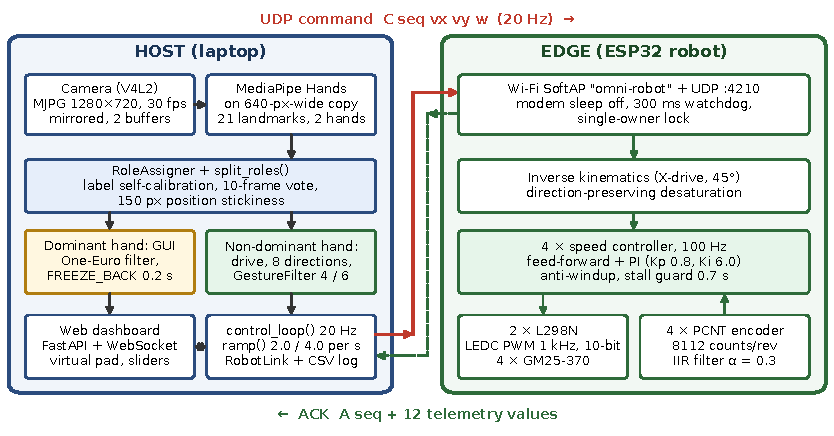
\includegraphics[width=0.86\textwidth]{fig_arch_en.pdf}
  \caption{Host--edge architecture. Solid red: UDP command; dashed green: acknowledgement with wheel telemetry.}
  \label{fig:arch}
\end{figure*}

\subsection{Kinematic Model}
Body velocity follows the ROS convention (Fig.~\ref{fig:kin}): $+x$ forward, $+y$ left, $+\omega$ counter-clockwise. Let $\mathbf{u}=[v_x, v_y, \omega]^{\top}\in[-1,1]^3$ be the normalized body command and $\mathbf{r}=[r_{FL}, r_{FR}, r_{RL}, r_{RR}]^{\top}$ the wheel speeds, where $1.0$ corresponds to $4300$ encoder counts per second. For the $45^{\circ}$ X-configuration the firmware uses
\begin{equation}
\mathbf{r}'=\begin{bmatrix}1&-1&-1\\1&1&1\\1&1&-1\\1&-1&1\end{bmatrix}\mathbf{u},\qquad
r_i=\frac{r'_i}{\max\!\left(1,\max_j |r'_j|\right)}.
\label{eq:ik}
\end{equation}
The common divisor keeps the direction of motion when one wheel would exceed its limit, which independent clipping would distort. The columns of the matrix in (\ref{eq:ik}) are orthogonal with squared norm $4$, so its pseudo-inverse is the transpose divided by four \cite{lynch2017} and the body velocity is recovered from the measured wheel speeds $\mathbf{m}$ by
\begin{equation}
\begin{bmatrix}v_x\\v_y\\\omega\end{bmatrix}_{\text{odo}}=\frac14\begin{bmatrix}1&1&1&1\\-1&1&1&-1\\-1&1&-1&1\end{bmatrix}\mathbf{m}.
\label{eq:fk}
\end{equation}
The robot uses four GM25-370 motors with a $1{:}78$ gearbox and Hall encoders. Counting both edges of both channels gives $8112$ counts per wheel revolution. The pulse-counter peripheral (PCNT) of the ESP32 decodes them in hardware with a $12.5\,\mu\mathrm{s}$ glitch filter \cite{esp32trm}.

\begin{figure}[!t]
  \centering
  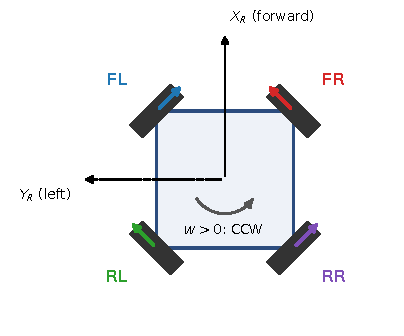
\includegraphics[width=0.62\columnwidth]{fig_kin_en.pdf}
  \caption{X-configuration geometry. Arrows give the thrust direction of each wheel for positive wheel speed.}
  \label{fig:kin}
\end{figure}

%--------------------------------------------------------------------
\section{Gesture Interface and Wheel Control}
\subsection{Finger State and Pointing Direction}
For each hand the 21 landmarks $p_k$ are used. A finger $f$ is extended when its fingertip is farther from the wrist than its proximal interphalangeal joint by a ratio that does not depend on the hand's distance to the camera or its in-plane rotation:
\begin{equation}
S(f)=\begin{cases}1,&\dfrac{\|p_{\mathrm{tip}(f)}-p_0\|_2}{\|p_{\mathrm{pip}(f)}-p_0\|_2}>1.15,\\[6pt] 0,&\text{otherwise.}\end{cases}
\label{eq:ext}
\end{equation}
If only the index finger is extended, the pointing angle is measured from the index base $p_5$ to the tip $p_8$ in the image plane and quantized to eight $45^{\circ}$ sectors, giving forward, backward, left, right and four diagonals. Index and middle fingers together pointing left or right command rotation. A fist or an open palm stops the robot. A \texttt{GestureFilter} requires $4$ consecutive frames to start a motion command and $6$ frames to stop.

\subsection{Hand Roles}
Because the displayed image is mirrored, the handedness label of MediaPipe is inverted from the user's point of view. The role assigner works in three cases. With two hands, roles follow the horizontal order of the wrists, and the disagreement between this order and the (flipped) labels updates a score $c_k=0.95\,c_{k-1}\pm0.05$; when $c_k<-0.6$ the flip convention is toggled. With one hand, the label is voted over the last $10$ frames. If a second hand has just disappeared and the remaining wrist moved by less than $150\,\mathrm{px}$, the previous role is kept. In manual mode the drive branch is disabled and any single hand is the UI hand, so the whole dashboard can be used with one hand.

\subsection{Cursor, Click Anchor and Slider Grab}
The index fingertip position is smoothed with a One-Euro filter \cite{casiez2012} with $f_{\min}=1\,\mathrm{Hz}$ and $\beta=8$ in normalized image units: the cut-off $f_c=f_{\min}+\beta|\dot{x}|$ is low when the hand is still and rises with speed. The UI hand has three poses: \emph{point} (index only; the cursor moves and a dwell of $0.8\,\mathrm{s}$ clicks), \emph{click} (index and middle; a click or a drag) and \emph{idle}. A pose must persist for $3$ frames.

Extending the middle finger can pull the index fingertip away from the intended target (Section~IV-B measures how much). When the pose changes from point to click at time $t$, the filtered point history $H$ gives the anchor
\begin{align}
(x_a,y_a)&=\bigl(x_j,y_j\bigr)\ \text{with}\ j=\arg\max\{t_j:\ t-t_j\ge 0.2\,\mathrm{s}\},\nonumber\\
(\Delta x,\Delta y)&=(x_a-x(t),\;y_a-y(t)),\label{eq:anchor}
\end{align}
and the action point used to hit the DOM element is $(a_x,a_y)=\mathrm{clamp}\bigl(x+\Delta x,\;y+\Delta y\bigr)$ while the click lasts. The displayed cursor still follows the fingertip, so dragging moves normally; after release the offset decays exponentially with a time constant of $0.15\,\mathrm{s}$. Sliders are grabbed by holding still on them, then moved relative to the finger motion, and released by holding still again.

\textbf{Mapping near the frame edge.}\label{sec:edge} Hand detection fails when the hand is cut by the frame border, so a cursor that coincides with the fingertip cannot reach the corners of the screen. Let $d=f-\tfrac12$ be the fingertip position in the frame ($f\in[0,1]$, per axis), $a=0.10$ the half width of the central zone and $b=0.44$ the distance at which the cursor should reach the screen edge. With $k=(0.5-b)/(b-a)^2$ the stretched coordinate is $s=\tfrac12+\operatorname{sgn}(d)\min\{\tfrac12,\ |d|+k(|d|-a)^2\}$ for $|d|>a$ and $s=f$ otherwise, which keeps the cursor on the fingertip in the middle, grows the lead smoothly without a kink (peak gain $1.35$) and reaches the screen edge when the fingertip is $6\,\%$ of the frame from the border. If the hand is lost while the fingertip is within $12\,\%$ of the border, the cursor and pose are held for $1.0\,\mathrm{s}$ instead of $0.3\,\mathrm{s}$. A first version, with a linear ramp starting at $|d|=0.30$ and peak gain $1.67$, made the cursor visibly run ahead of the fingertip and was replaced by this one. Nine of the $55$ automatic checks cover this mapping.

\subsection{Per-Wheel Speed Control}
Two limiters guard against slip and supply sag. On the host, the body command ramps with at most $2.0\,\mathrm{s^{-1}}$ acceleration and $4.0\,\mathrm{s^{-1}}$ deceleration, and passes through zero before changing sign. On the ESP32 every wheel target moves toward its goal at most $4.0\,\mathrm{s^{-1}}$.

At every $10\,\mathrm{ms}$ step $k$, wheel $i$ has the filtered measured speed $\omega_i(k)=0.7\,\omega_i(k-1)+0.3\,c_i(k)/4300$, with $c_i$ the counts per second. The control law, a feed-forward term plus a PI term with conditional anti-windup \cite{astrom2006}, is
\begin{align}
u^{\mathrm{ff}}_i&=\operatorname{sgn}(r_i)\bigl(a_i+b_i|r_i|\bigr),\quad e_i=r_i-\omega_i,\nonumber\\
I_i&\leftarrow I_i+K_i e_i\,\Delta t\ \ \text{only if not ramping and not saturated},\nonumber\\
u_i&=\mathrm{clamp}\bigl(u^{\mathrm{ff}}_i+K_p e_i+I_i,\,-1,\,1\bigr),\label{eq:ctrl}
\end{align}
with $K_p=0.8$, $K_i=6.0$. The constants $a_i$ and $b_i$ are least-squares fits of the steady-state duty versus speed measured with the wheels lifted (Table~\ref{tab:ff}). A wheel whose duty is at least $0.95$ while its speed stays below $0.05$ for $0.7\,\mathrm{s}$ is switched off to protect against a jam.

\begin{table}[!t]
\caption{Identified feed-forward parameters (wheels lifted) and mean steady tracking error on the floor.}
\label{tab:ff}
\centering
\small
\begin{tabular}{lcccc}
\toprule
Wheel & $a_i$ & $b_i$ & \multicolumn{2}{c}{Mean error (\%)} \\
 & (duty) & & v1 gest. & v2 two-hand \\
\midrule
FL & 0.076 & 0.470 & 1.9 & 2.5 \\
FR & 0.148 & 0.594 & 2.5 & 2.6 \\
RL & 0.055 & 0.453 & 1.6 & 2.3 \\
RR & 0.060 & 0.464 & 1.7 & 2.5 \\
\bottomrule
\end{tabular}
\end{table}

%--------------------------------------------------------------------
\section{Experiments}
\subsection{Setup}
The host is a laptop with an Intel Core i5-13420H (12 threads, 15\,GB RAM) running Linux, Python 3.12, MediaPipe 1.2.0 (CPU) and OpenCV 5.0. The robot is an ESP32 DevKit V1 with two L298N modules, four GM25-370 motors and a $12\,\mathrm{V}$ supply. Three runs on a floor were logged at $20\,\mathrm{Hz}$ (Table~\ref{tab:data}); the first two use the single-hand version (v1) and the third the dual-hand version (v2). In the manual run, $389$ of the logged rows belong to gesture mode. Rows recorded while the motor supply was off ($53$ rows in the manual run) are excluded. Only one operator and one robot were used. The dashboard is described in the accompanying technical report.

\begin{table}[!t]
\caption{Logged runs. RTT is the UDP round-trip time: median / 95th percentile / maximum.}
\label{tab:data}
\centering
\small
\begin{tabular}{lrrr}
\toprule
Run & Rows & Time (s) & RTT (ms) \\
\midrule
Manual (v1)   & 3240 & 1512 & 7.8 / 22.5 / 97 \\
Gesture (v1)  & 4820 &  247 & 8.1 / 26.1 / 101 \\
Two-hand (v2) & 5020 &  266 & 6.6 / 16.1 / 909 \\
\midrule
Total & 13080 & 2026\textsuperscript{a} & -- \\
\bottomrule
\multicolumn{4}{l}{\footnotesize\textsuperscript{a}Sum of the unrounded durations.}
\end{tabular}
\end{table}

\subsection{Vision Pipeline}
Camera and inference speed were measured on $359$ consecutive frames with the full capture-and-detect loop and no hand in view: $29.9$ fps, with a hand-landmark inference time of $18.5\,\mathrm{ms}$ (mean), $18.2\,\mathrm{ms}$ (median), $27.1\,\mathrm{ms}$ (95th percentile). The cost with hands present is given in Section~IV-E. Setting the driver buffer to one frame instead of two halved the stream from $28.9$ to $14.5$ fps in an earlier benchmark with MJPG, because the camera dropped frames while the application held the only buffer.

The geometric logic is covered by $55$ automatic checks on synthetic hands (gestures, pose, role assignment including inverted labels, cursor) and $49$ checks of the dashboard's cursor handling in a browser (headless Chrome, $1280\times900$ window) (dwell click, two-finger click, relative slider grab, pad drag, hold buttons, release on lost hand); all passed on 12 November 2026.

In the two real gesture runs the filtered gesture changed $120$ and $76$ times; $7$ ($5.8\,\%$) and $5$ ($6.6\,\%$) of these lasted less than $0.3\,\mathrm{s}$, i.e., $94.2\,\%$ and $93.4\,\%$ of gesture segments were stable by this criterion. Whether the short segments were unintended was not annotated.

\emph{Cursor: a negative result.} A simulated hand suggested large benefits: with $2\,\mathrm{px}$ Gaussian noise ($200$ seeded runs) the filter cut the horizontal standard deviation of the cursor by $65.5\,\%$, and the click anchor cut the action-point shift by $83.6\,\%$ for a $29.2\,\mathrm{px}$ fingertip jump.

On a real hand (script \texttt{tests/real\_hand\_eval.py}, one operator, $640\times480$ frames) neither effect was reproduced. With the index finger held still for $8\,\mathrm{s}$ ($209$ frames) the standard deviation of the raw fingertip was $2.26\,\mathrm{px}$ and that of the filtered cursor $2.14\,\mathrm{px}$ ($-5\,\%$); real tremor is probably slow and correlated, which a low-pass filter tuned for responsiveness does not remove (not tested). For the click shift, the operator held the fingertip still (within $3\,\mathrm{px}$ for $1\,\mathrm{s}$, drifting trials rejected) and raised the middle finger $12$ times. The fingertip moved by a median of only $1.65\,\mathrm{px}$ ($1.1$--$5.7$), against $29.2\,\mathrm{px}$ in the simulation, and the action point with the anchor moved by a median of $4.15\,\mathrm{px}$ ($2.0$--$12.0$), more than the fingertip in $11$ of $12$ trials (Fig.~\ref{fig:real}), so the $0.2\,\mathrm{s}$ look-back added about $2.5\,\mathrm{px}$ instead of removing a shift. An earlier run in which the operator did not keep the finger still is not used. With $12$ clicks from one operator and no click hit-rate measurement, this is indicative only; the dwell radius ($30\,\mathrm{px}$) and the button sizes exceed these shifts, so the practical effect on clicking is probably small but untested.

\begin{figure}[!t]
  \centering
  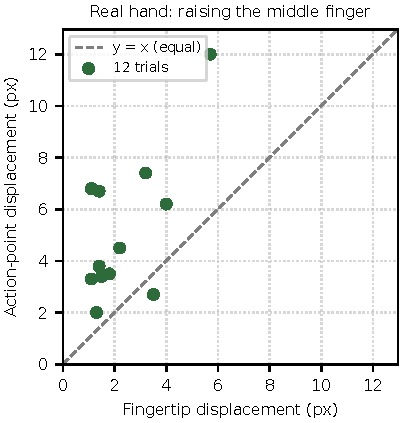
\includegraphics[width=0.78\columnwidth]{fig_real_en.pdf}
  \caption{Real hand, 12 trials with the finger held still: displacement of the action point against that of the raw fingertip when the middle finger is raised. Points above the dashed line mean the action point moved more than the fingertip.}
  \label{fig:real}
\end{figure}

\subsection{Link Latency}
The round-trip time is measured per command from the sequence number of the UDP command to that of its acknowledgement. Table~\ref{tab:data} and Fig.~\ref{fig:rtt}(a) show medians of $6.6$--$8.1\,\mathrm{ms}$ and a heavy tail; the worst single value, $909\,\mathrm{ms}$ in the two-hand run, is far above the $300\,\mathrm{ms}$ robot watchdog and so a stop would have occurred. This is round-trip network latency only; it excludes camera capture, inference and gesture filtering.

For $38$ ($26$) confirmed motion gestures in the v1 gesture (v2) run, the time from the logged gesture to the moment the most loaded wheel reached $50\,\%$ of its new target was $260\,\mathrm{ms}$ median ($204$--$359\,\mathrm{ms}$) and $257\,\mathrm{ms}$ median ($203$--$309\,\mathrm{ms}$). This includes the deliberate acceleration limits of Section~III-D, so it is not the minimum achievable latency, and it does not include the $4$ frames ($\approx133\,\mathrm{ms}$) needed to confirm a gesture.

\begin{table*}[!t]
\caption{Commanded vs. encoder-derived body velocity (normalized units). The first six primitives are from the v1 gesture run; the diagonals are from the v2 run.}
\label{tab:odo}
\centering
\footnotesize
\setlength{\tabcolsep}{3pt}
\begin{tabular}{lrcccc}
\toprule
Primitive & Samples & Command $(v_x,v_y,\omega)$ & From encoders $(v_x,v_y,\omega)$ & Main-axis error & Max other axis \\
\midrule
Forward        & 543 & (+0.472, 0.000, 0.000) & (+0.474, +0.001, +0.002) & +0.6\,\% & 0.002 \\
Backward       & 360 & (-0.510, 0.000, 0.000) & (-0.510, -0.001, -0.001) & -0.1\,\% & 0.001 \\
Left           &  96 & (0.000, +0.480, 0.000) & (+0.004, +0.482, +0.002) & +0.4\,\% & 0.004 \\
Right          &  73 & (0.000, -0.480, 0.000) & (-0.003, -0.479, 0.000) & -0.2\,\% & 0.003 \\
Rotate left    & 238 & (0.000, 0.000, +0.435) & (+0.003, +0.001, +0.446) & +2.5\,\% & 0.003 \\
Rotate right   & 230 & (0.000, 0.000, -0.442) & (-0.001, 0.000, -0.453)  & +2.4\,\% & 0.001 \\
Forward-left (v2)  &  98 & (+0.308, +0.245, 0.000) & (+0.316, +0.256, +0.001) & -- & -- \\
Forward-right (v2) &  71 & (+0.313, -0.237, 0.000) & (+0.316, -0.243, -0.002) & -- & -- \\
\bottomrule
\end{tabular}
\end{table*}

\begin{figure*}[!tb]
  \centering
  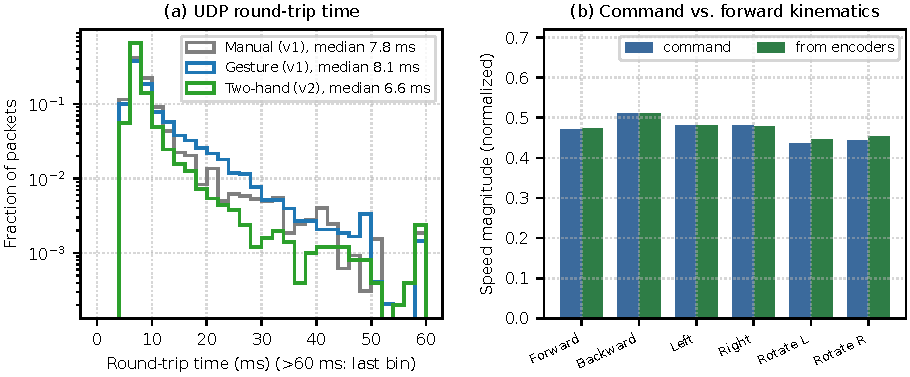
\includegraphics[width=0.8\textwidth]{fig_rtt_odo_en.pdf}
  \caption{(a) Distribution of the UDP round-trip time for the three runs (log scale; values above $60\,\mathrm{ms}$ fall into the last bin). (b) Magnitude of the commanded and the encoder-derived velocity for the six primitives.}
  \label{fig:rtt}
\end{figure*}

\begin{figure*}[!tb]
  \centering
  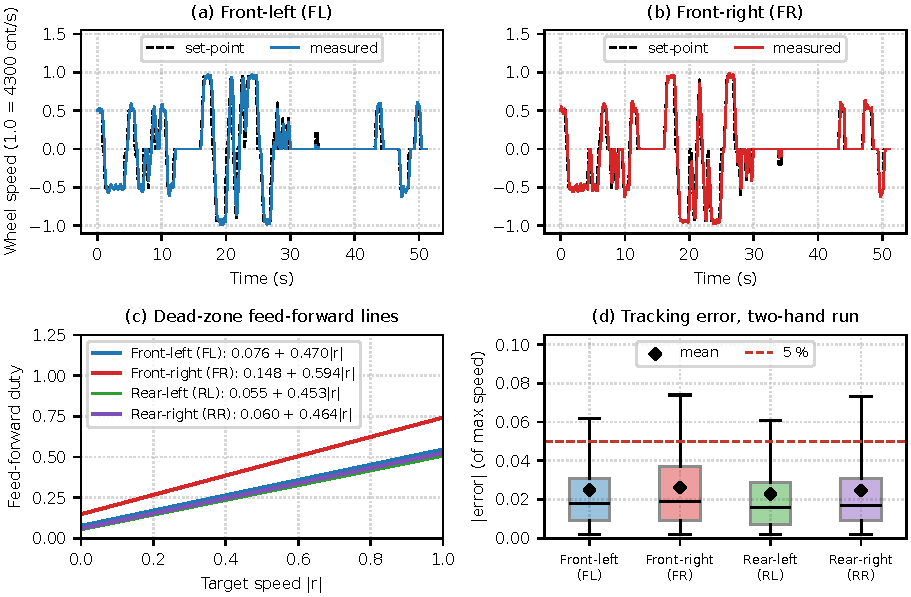
\includegraphics[width=0.72\textwidth]{fig_wheel_en.pdf}
  \caption{Wheel-speed control in the two-hand run. (a),(b) Set-point and measured speed for two wheels over a $50\,\mathrm{s}$ window. (c) Identified feed-forward lines. (d) Distribution of the steady-state tracking error (whiskers: 5th--95th percentile; diamond: mean); the dashed line marks $5\,\%$.}
  \label{fig:wheel}
\end{figure*}

\subsection{Wheel Tracking and Body Motion}
We evaluate wheel tracking only when the command has been constant for $0.3\,\mathrm{s}$ and at least $0.1$ in magnitude. Table~\ref{tab:ff} and Fig.~\ref{fig:wheel} give mean errors of $1.5$--$3.2\,\%$ of full scale over the three runs. The $95$th percentile of the error is higher, $4.4$--$4.8\,\%$ in the v1 gesture run and $6.1$--$7.4\,\%$ in the v2 run, so the $5\,\%$ mark is met by the mean but not by the tail in the latter. The front-right wheel, which has the largest dead zone, needs the highest mean duty ($0.48$--$0.49$ against $0.36$--$0.44$). We did not compare against a plain PID or against open loop on the same trajectories, so the benefit of the proposed controller over those is not quantified here.

Table~\ref{tab:odo} compares the commanded and the encoder-derived body velocity from (\ref{eq:fk}) over segments with a constant primitive. The error in the main axis is below $0.6\,\%$ for translations and about $2.4$--$2.5\,\%$ for rotations, and the unintended motion in the other axes stays at or below $0.004$. These are velocities from the wheel encoders and do not include wheel slip on the floor, so they are not ground-truth position errors.

\subsection{Second Session: Vision Loop with Hands, End-to-End Latency and the Cursor near the Frame Edge}
After the runs above we recorded four more server sessions with the per-run logger (\texttt{web/runlog.py}): one log row per camera frame, plus the 20\,Hz drive log when the robot was connected (data in \texttt{docs/data/v2/session2/}, table~\ref{tab:sess2}). Sessions A and B ran the code from before the changes described below (MJPG $640\times480$ capture, cursor mapped 1:1 to the fingertip); sessions C and D ran after the capture was raised to $1280\times720$ (hand detection still on a $640$-px-wide copy) and after the cursor was made to move faster than the fingertip near the frame edge (C with a piecewise-linear mapping, D with the smooth mapping of Section~\ref{sec:edge}). A and B had the robot connected; C and D tested the cursor only. A is the first run after a wheel fault was repaired, and D was still running when its log was copied, so D is a snapshot. One operator took part in all four sessions, and the sessions differ in what the operator did, in the number of open browser tabs and in duration, so they are not a controlled comparison.

\begin{table}[!t]
\caption{Server sessions recorded with the per-run logger. Mean hand-landmark inference time (ms) is split by the number of hands in the frame; fps is the number of AI frames per second over the whole session.}
\label{tab:sess2}
\centering
\footnotesize
\setlength{\tabcolsep}{3pt}
\begin{tabular}{llcrrrrr}
\toprule
Sess. & Camera & Cursor & Time (s) & fps & 0 hand & 1 hand & 2 hands \\
\midrule
A & 640$\times$480 & 1:1 & 186 & 25.5 & 27.7 & 45.5 & 43.3 \\
B & 640$\times$480 & 1:1 & 76 & 21.9 & 31.3 & 50.1\textsuperscript{a} & 47.5 \\
C & 1280$\times$720 & piecewise & 363 & 18.0 & 30.7 & 55.5 & 48.3 \\
D & 1280$\times$720 & smooth & 214 & 21.9 & 28.9 & 52.4 & 47.2 \\
\bottomrule
\multicolumn{8}{l}{\footnotesize\textsuperscript{a}Only 46 frames with exactly one hand.}\\
\end{tabular}
\end{table}

\emph{Vision loop with hands.} With no hand in view, inference averaged $27.7$--$31.3$\,ms; with one hand $45.5$--$55.5$\,ms and with two hands $43.3$--$48.3$\,ms (Fig.~\ref{fig:sess2}a). The frame rate over a whole session was $18.0$--$25.5$ fps, below the 25 fps target and below the 29.9 fps of the isolated benchmark above, which measured capture and detection alone with no hand; the server also encodes and streams every frame and runs the control loop, and the cause of the difference was not isolated. Frames with one hand were not cheaper than frames with two (a possible reason, that the detector keeps searching for the missing second hand, was not tested). Raising the capture to $1280\times720$ did not change the no-hand cost ($27.7$--$31.3$\,ms in all four sessions); with one hand the mean was higher in C and D than in A ($55.5$ and $52.4$ against $45.5$\,ms), but the sessions are not comparable enough to attribute this to the resolution.

\begin{figure*}[!tb]
  \centering
  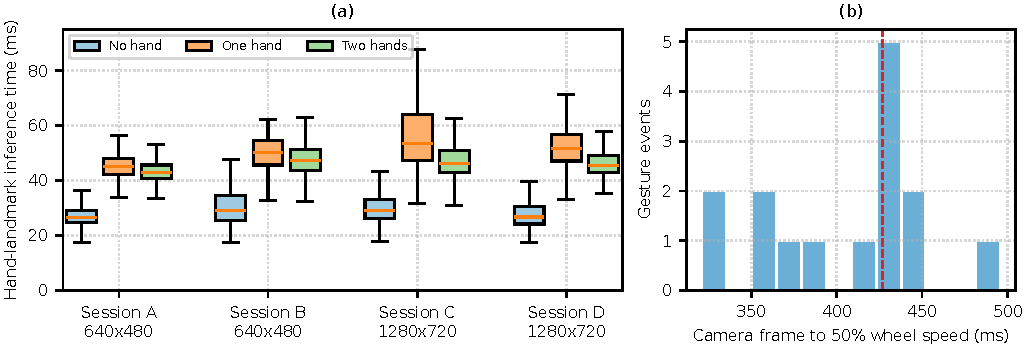
\includegraphics[width=0.8\textwidth]{fig_sess2_en.pdf}
  \caption{(a) Hand-landmark inference time per session and number of hands in view (boxes: quartiles; whiskers without outliers). (b) Delay from the camera frame in which the gesture filter confirmed a motion gesture to the moment the most loaded wheel reached 50\,\% of its new target, session A (15 events; dashed: median).}
  \label{fig:sess2}
\end{figure*}

\emph{End-to-end latency (session A).} For $15$ confirmed motion gestures, the median time from the camera frame in which the gesture filter fired to the moment the most loaded wheel reached 50\,\% of its new target was $427$\,ms ($321$--$496$\,ms, Fig.~\ref{fig:sess2}b); the command left the laptop $37$\,ms after that frame (median). The filter itself needs $4$ consecutive frames, about three frame intervals ($120$--$140$\,ms at these frame rates) before the confirming frame, which is not included. The median target magnitude was $0.81$ of full speed; with the host acceleration limit of $2.0\,\mathrm{s^{-1}}$ half of that takes about $0.2\,\mathrm{s}$, so a large part of the delay is the deliberate ramp. This is longer than the $257$--$260\,\mathrm{ms}$ reported in Section~IV-C, which started from the gesture value written in the drive log instead of the camera frame (about $37$\,ms later) and used targets of other sizes; the $15$ events here are too few and too uniform to separate these causes. Session B contains a single event ($319$\,ms, target $0.5$).

\emph{Wheel tracking and link.} With the same rule as in Section~IV-D, the mean error was $1.3$\,\% (manual) and $1.5$\,\% (gesture) of full scale in A, and $0.9$\,\% in B (gesture only; $12$ manual samples are too few to report), with $95$th percentiles of $4.3$, $5.0$ and $4.2$\,\%. In A the duty was at the $0.95$ ceiling in $8.0$\,\% of the manual and $3.8$\,\% of the gesture samples, against $0.0$\,\% in B: at the higher speeds of A the controller ran out of voltage headroom, so the commanded speed could not be reached, which can distort diagonal motion if the wheels saturate unequally (not measured). The UDP round trip had a median of $6.4$ and $7.9$\,ms (95th percentile $23.9$ and $17.3$\,ms; maximum $104$ and $47$\,ms), consistent with the earlier runs.

\emph{Cursor near the frame edge.} The mapping of Section~\ref{sec:edge} was introduced after the operator reported that the UI hand was lost whenever the fingertip had to reach the frame border to hit the speed slider in the screen corner, and then that the cursor ran ahead of the fingertip when the stretch started abruptly. The logs give an indirect view only, because they do not store the raw fingertip position: the share of UI-hand frames with the cursor within $2\,\%$ of a screen edge was $2.3$\,\% in A and $1.4$\,\% in B (1:1 mapping), and $8.2$\,\% in C and $4.6$\,\% in D (stretched); the number of UI-hand segments longer than $0.3\,\mathrm{s}$ that ended with the cursor at an edge, a sign of losing the hand there, was $1$ of $6$ in A, $1$ of $3$ in B, $0$ of $15$ in C and $1$ of $9$ in D. The operator also needed the corner more in C and D because the task was to reach it, so these numbers show that the cursor reaches the screen edge with the stretched mapping, not that hand loss was reduced; the counts are small. The lead of the cursor over the fingertip near the edge (up to $6\,\%$ of the frame width by construction) was not measured against the fingertip position and rests on the operator's report.

%--------------------------------------------------------------------
\section{Limitations}
The results come from one robot on one floor with one operator. There is no user study, so the claim that the interface is more convenient than a mouse is untested. The real-hand cursor measurements (jitter, click shift) come from one operator and $12$ clicks, and the click hit rate was not measured. The comparison of the controller with a baseline is missing, and the gesture stability criterion does not tell intended from unintended transitions. The end-to-end latency was measured in one session ($15$ events), and the effect of the edge mapping on hand loss was not measured against the true fingertip position. The system has no obstacle sensing: the operator is the only safeguard.

\section{Conclusion}
A single webcam and a single ESP32 sufficed to operate a four-wheel omnidirectional robot and its dashboard at the same time: one hand for the interface and the other for driving. On the logged runs the link round trip was a few milliseconds at the median, the mean wheel-speed error was $1.5$--$3.2\,\%$ of full scale, and the encoder-derived body motion agreed with the commands within $2.5\,\%$. In later sessions with real hands the vision loop ran at $18.0$--$25.5$ fps and the median delay from the camera frame to half wheel speed was about $427$\,ms, so the interactive latency, not the link, is the limit to improve. The click anchor and the filter parameters need revisiting given the real-hand measurements. Planned work is a user study with real hands, a comparison with baseline controllers, a heading sensor, and obstacle sensing.

\FloatBarrier
\begin{thebibliography}{00}
\bibitem{siegwart2011} R.~Siegwart, I.~R. Nourbakhsh, and D.~Scaramuzza, \emph{Introduction to Autonomous Mobile Robots}, 2nd~ed. Cambridge, MA, USA: MIT Press, 2011.
\bibitem{zhang2020} F.~Zhang \emph{et al.}, ``MediaPipe Hands: On-device real-time hand tracking,'' arXiv:2006.10214, 2020 (CVPR Workshop on Computer Vision for AR/VR).
\bibitem{casiez2012} G.~Casiez, N.~Roussel, and D.~Vogel, ``1\texteuro{} filter: A simple speed-based low-pass filter for noisy input in interactive systems,'' in \emph{Proc. ACM CHI}, Austin, TX, USA, 2012, pp. 2527--2530.
\bibitem{lynch2017} K.~M. Lynch and F.~C. Park, \emph{Modern Robotics: Mechanics, Planning, and Control}. Cambridge, U.K.: Cambridge Univ. Press, 2017.
\bibitem{astrom2006} K.~J. {\AA}str{\"o}m and T.~H{\"a}gglund, \emph{Advanced PID Control}. Research Triangle Park, NC, USA: ISA, 2006.
\bibitem{esp32trm} Espressif Systems, ``ESP32 Technical Reference Manual,'' (pulse counter and LED PWM controller chapters).
\end{thebibliography}

\end{document}
